\chapter{Sviluppo}
In questo capitolo verrà descritto il processo di sviluppo
seguito per l'implementazione di \pygfa, analizzandone le
fasi principali, descrivendo i problemi incontrati e come sono stati
affrontati. Verrà infine fornito un caso di esempio che mostra
le funzionalità della libreria.

\section{Processo}
Lo scopo di \pygfa è quello di fornire un ambiente per lo sviluppo
di applicativi in grado di analizzare e manipolare file GFA. Non
è pertanto un prodotto finito, con casi d'uso definiti e risultati attesi
con cui è possibile confrontare i risultati. Non si è ritenuto appropriato,
di conseguenza, seguire un processo di sviluppo con fasi di analisi
e pianificazione profonde, che con il mutare dei requisti (per la
maggior parte non definiti fin dall'inizio) avrebbero potuto
compromettere la struttura del sistema. Un altro fattore da
tenere in considerazione è che le mie conoscenze sul significato
che i dati contenuti nei file GFA e le considerazioni che si potevano dedurre
da esse sono cresciute con lo sviluppo del sistema stesso. Perciò un'analisi,
anche se non approfondita, non poteva essere svolta a priori; poiché
avrebbe potenzialmente comportato una serie di ritardi
nello sviluppo del progetto dovute allo studio dei concetti biologici
che avrebbe richiesto diverso tempo.


Per questi motivi, il processo di sviluppo che si è deciso di utilizzare è di \emph{extreme}
\emph{programming}; con fasi di analisi e pianificazione molto veloci,
dando priorità all'implementazione delle parti essenziali del sistema aventi
maggior priorità per poi ripetere il procedimento con l'evolversi dei
requisiti e delle funzionalità richieste, cercando di avere un riscontro
costante con i clienti finali (in questo caso i referenti della tesi).

Affiancata alla parte di implementazione si è svolta la parte di testing,
che purtroppo non si è riusciti a condurre esattamente nella forma di Test Driven
Development, ma alla quale è stata data comunque una priorità molto alta
sia per la verifica delle funzionalità dei metodi, che per la verifica della
presenza di errori nel codice, che nel contesto di un linguaggio non compilato,
quale è il Python, risulta una pratica molto importante per garantire il
corretto funzionamento del programma.

Nel complesso si è riusciti a seguire abbastanza rigorosamente questi cicli
di pianificazione veloce, implementazione e test; procedendo al termine
di ogni ciclo con una fase di refactoring del codice e di miglioramento
della documentazione presente in esso, avvalendosi di Pylint per individuare
quelle porzioni di codice che era possibile migliorare.

\subsection{Fasi di sviluppo}
La rappresentazione delle informazioni contenute nei file GFA subisce
diverse trasformazioni prima di giungere come dato di un nodo, arco o
sottografo presente in un oggetto grafo GFA. L' iniziale rappresentazione
testuale di ogni linea viene rappresentata da una classe che ne indica
il tipo e i valori dei campi che contiene. Successivamente le linee
vengono convertite in archi, nodi o sottografi e infine nodi e archi
vengono rappresentati mediante dizionari Python, una volta inseriti
effettivamente nel grafo. Quest'ultima trasformazione è stata
adottata per uniformarsi al trattamento dei dati di un grafo in modo analogo
al modo in cui NetworkX li gestisce, garantendo una facilità di accesso
alle informazioni ed evitando che l'utente finale debba adattarsi ad un
nuovo modo di operare.

\'E possibile suddividere lo sviluppo di \pygfa in tre fasi principali:
\begin{itemize}
	\item sviluppo del parser;
	\item progettazione delle classi di astrazione dei dati GFA;
	\item sviluppo della classe del grafo GFA e delle operazioni che è
		possibile eseguire su di esso.
\end{itemize}
\captionsetup{justification=centering}
\begin{figure}[h]
	\centering
	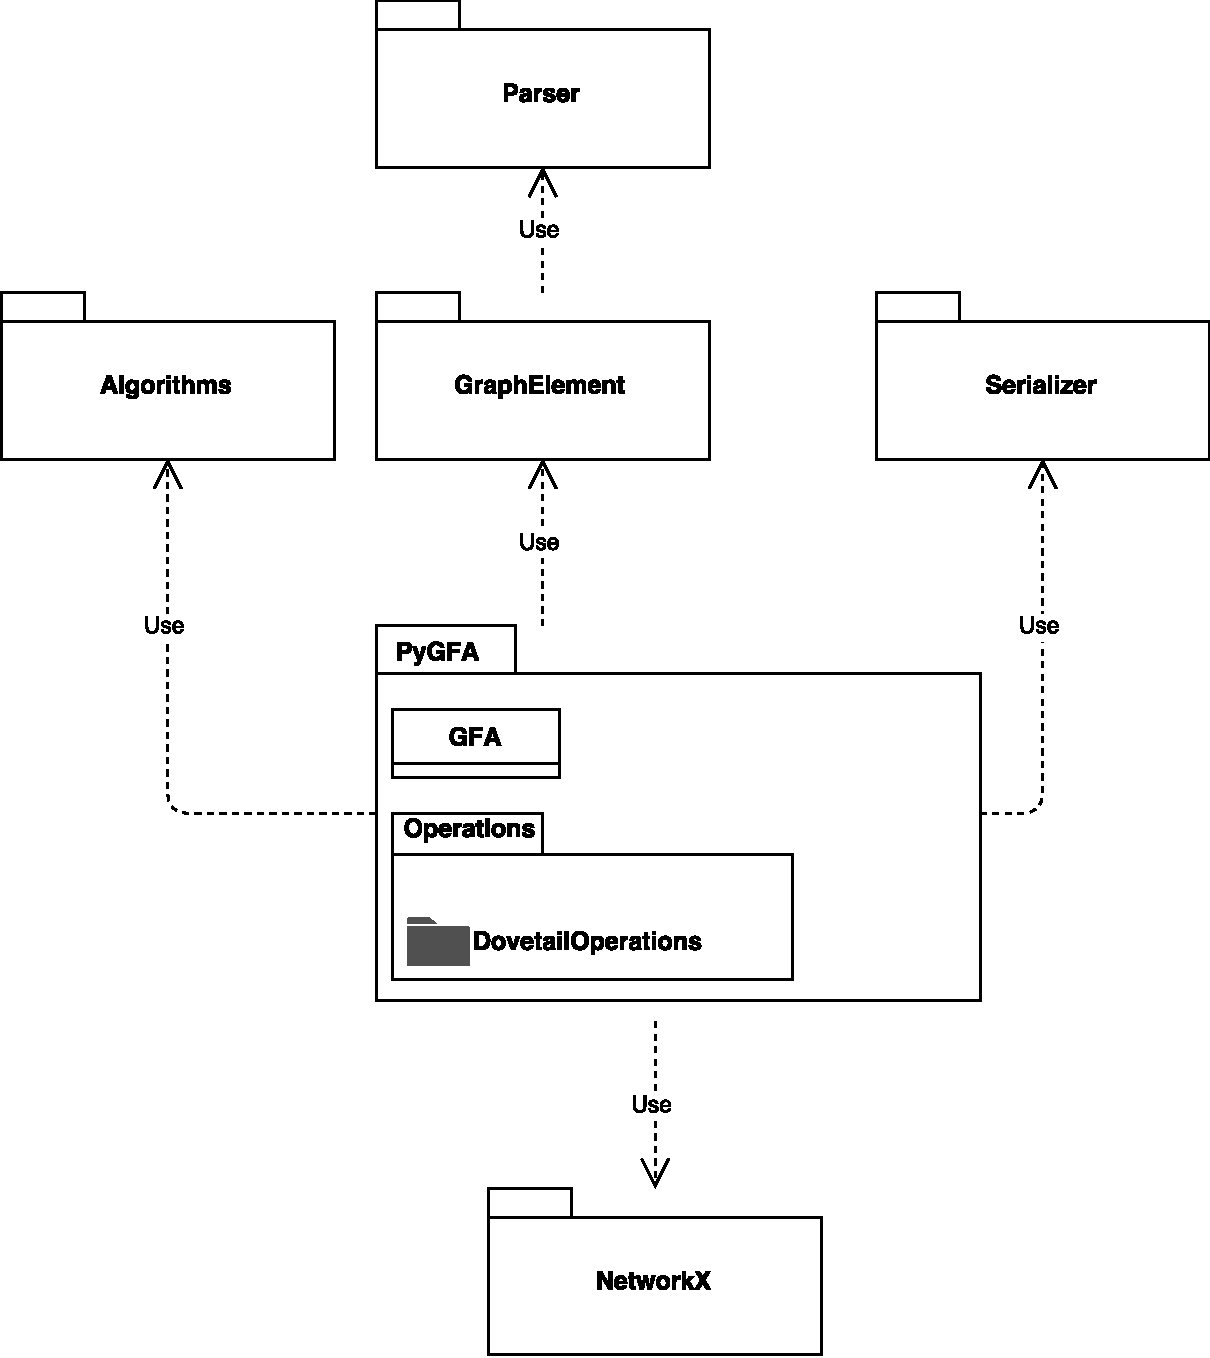
\includegraphics[scale=0.5]{package_diagram}
	\caption[Diagramma dei package]{Diagramma dei package di \pygfa.}
\end{figure}
\captionsetup{justification=justified}

Il parser si occupa di leggere le linee di un file GFA, di verificare la correttezza
sintattica dei suoi campi e di rappresentarne le informazioni mediante una classe
specifica per ogni tipo di linea.

Nella seconda fase si sono analizzate le linee delle due specifiche e si
è stabilito come attribuire ad ogni linea un ruolo che potesse essere di
nodo, arco o sottografo del grafo GFA finale. Gli attributi delle classi
del grafo astraggono gli attributi delle linee delle specifiche, 
di conseguenza è stata necessaria
una pianificazione dell'assegnamento degli attributi delle linee ad
attributi degli elementi del grafo.

Nella fase finale si è sviluppata la classe del grafo GFA fornendo
metodi di inserimento, accesso ed eliminazione sui singoli elementi che
lo compongono e aggiungendo le interfacce agli algoritmi forniti da Networkx
per eseguire le operazioni sui dati GFA.

\section{Fase1: sviluppo del parser}
Per la scrittura del parser si è seguito un approccio \emph{bottom-up},
sviluppando dapprima le classi rappresentanti i campi,
che sono presenti in ogni linea, 
e successivamente descrivendo con una classe ciascun tipo
di linea presente nelle specifiche.

Il parser effettua solo un controllo sintattico sulle informazioni dei file
al fine di garantire una corretta gestione delle informazioni da parte
della libreria; non verifica eventuali incongruenze tra le informazioni
presenti. Per questo motivo si suppone che il file GFA che viene fornito
sia stato già validato da un punto di vista di namespace degli elementi
e di coerenza delle informazioni (per esempio il riutilizzo di un identificativo
già utilizzato da un altro elemento o riferimenti a elementi
che non vengono definiti).

Ogni campo di ogni linea, in entrambe le specifiche, può essere descritto
da un \emph{espressione regolare}. Per questo motivo è stato
implementato un modulo Python per la validazione di tutti i campi definiti
dalle specifiche, associando un nome ad ogni espressione e creando un metodo
\texttt{is\_valid} che, data una stringa e il nome del tipo di un campo,
verifica che la stringa rispetti l'espressione regolare indicata dal nome
del campo fornito.
Per rappresentare i campi delle linee sono state create due classi,
\texttt{Field} e \texttt{OptField}; la prima
descrive i campi obbligatori, per i quali non viene specificato
esplicitamente il tipo di dato che contengono; la seconda
descrive i campi opzionali per i quali sono forniti
nome (il tag), tipo e valore. Mentre nei campi opzionali
è possibile, fin dall'instanziazione dell'oggetto, effettuare una validazione
sul contenuto, sui campi obbligatori non è possibile, in quanto
la tipologia del loro contenuto assume valore solo nel contesto
della linea cui appartengono.

Successivamente si è modellata la classe \texttt{Line} dalla quale
derivano le classi rappresentanti le altre linee. Questa classe
racchiude due campi: \texttt{PREDEFINED\_OPTFIELDS}
e \texttt{REQUIRED\_FIELDS} che racchiudono i campi opzionali che
ogni linea può contenere e i campi obbligatori che necessita, rispettivamente.
Inoltre questa classe possiede i metodi di aggiunta e rimozione dei campi,
assicurandosi di validare il contenuto dei campi obbligatori nel contesto
di ciascuna linea. Le altre classi, derivando da questa, devono
ridefinire i propri campi opzionali predefiniti e i campi obbligatori oltre
a indicare un metodo per convertire una stringa
nel corrispettivo oggetto che la rappresenta, condividendo la stessa
logica di manipolazione e validazione dei campi che viene riutilizzata
grazie al \emph{polimorfismo}.

\captionsetup{justification=centering}
\begin{figure}[h]
	\centering
	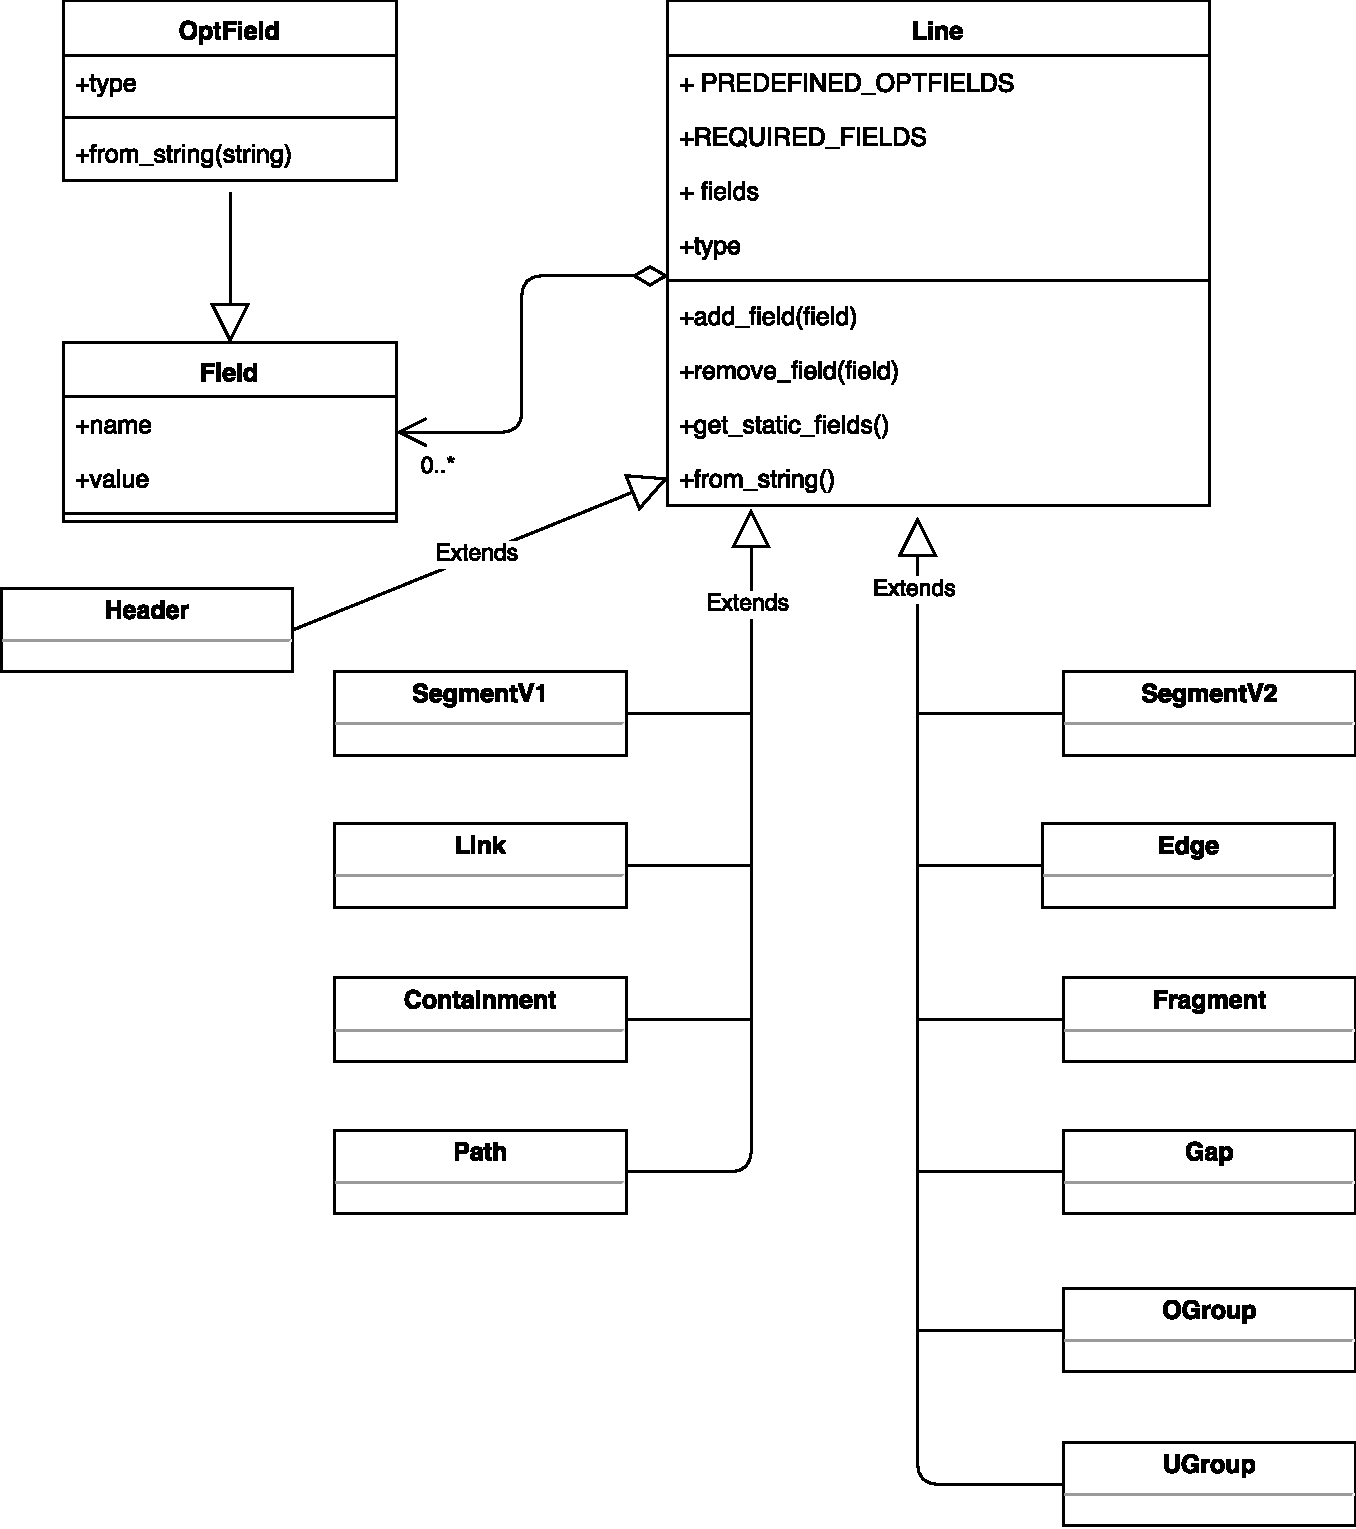
\includegraphics[scale=0.5]{parser_class_diagram}
	\caption[Diagramma delle classi del package parser]{Diagramma delle classi usate dal parser.}
\end{figure}
\captionsetup{justification=justified}
\clearpage

\section{Fase2: astrazione dei dati}
In questa fase sono state analizzate le singole informazioni presenti
nelle linee di entrambe le specifiche, evidenziandone gli aspetti simili al
fine di giungere ad una loro rappresentazione generalizzata per mezzo di tre
entità: \emph{Nodo}, \emph{Arco}, \emph{Sottografo}.

Ciascuna linea GFA può essere facilmente associata ad uno di questi tre
elementi. Nonostante sia possibile estendere GFA2 con nuovi tipi di linee, è bene notare
che questo lavoro di assegnazione di un ruolo ad ogni linea limita questa funzionalità
della specifica, in quanto sarebbe necessario capire il ruolo che queste nuove
linee possono ricoprire nei grafi di assemblaggio e ridefinire i meccanismi con
cui \pygfa riesce a manipolare queste nuove informazioni. \'E comunque possibile,
vista la mancanza dei concetti di visibilità privata del linguaggio, andare ad inserire
queste informazioni direttamente al grafo NetworkX che sta alla base dell'oggetto grafo
GFA, ma non è possibile garantire la consistenza delle operazioni che è possibile
effettuare usando la libreria.

Una sequenza costituisce il principale tipo di informazione cui si
è interessati, più sequenze sono in relazione da una serie di collegamenti descritti
dalle specifiche. Perciò possiamo attribuire alle sequenze (quindi alle linee Segment)
il ruolo di nodi.
La linea di header non contiene di per se informazioni che è possibile rappresentare
su di un grafo. Al momento \pygfa non modella le informazioni che possono essere
descritte dalle linee di header.

Tutte quelle linee che vedono come protagoniste due sequenze possono essere
considerate come degli archi che collegano due nodi $u$ e $v$. Appartengono
a tale insieme le linee di link, containment, edge, fragment e gap.

Le linee rimanenti: path, ogroup e ugroup, rappresentano tutte un insieme
(ordinato o meno) di nodi e archi che descrivono un sottografo composto
dagli elementi del file GFA; di conseguenza tali linee vengono considerate come
dei sottografi.

Visto che GFA2 è un superset di GFA1, si è analizzato come sarebbe stato
possibile rappresentare ciascuna linea di GFA1 nel corrispettivo elemento
di GFA2, capendo in questo modo gli attributi che ciascuna delle classi (Nodo, Arco
e Sottografo) avrebbe dovuto contenere per modellare quelle informazioni.
Terminato il confronto delle linee di GFA1 si sono aggiunte quelle
informazioni delle linee di GFA2 che non erano state prese in considerazione
(poiché non rappresentate) e le si sono andate ad aggiungere come attributi
aggiuntivi delle classi rappresentanti gli elementi del grafo.
Le informazioni che diventeranno attributi espliciti delle classi sono date
esclusivamente dai campi obbligatori di ciascuna linea, per entrambe le
classi i dati provenienti da campi opzionali verranno memorizzate
all'interno di un dizionario Python e indicate da un unico campo
\texttt{opt\_fields}; si noti che nonostante il nome, i campi contenuti
non sono (solamente) riferimenti ai campi opzionali delle specifiche,
ma si riferiscono ad una qualsiasi informazione
che l'utente vuole aggiungere all'elemento.

Di seguito verrà elencato ciascun campo di ogni linea, la relativa rappresentazione
in GFA2 e la scelta di come si è deciso di modellare tale campo nell'elemento
del grafo corrispondente. Per i nomi dei campi si farà riferimento alla nomenclatura
utilizzata dalla specifica per indicare ciascun campo, si noti
che alcuni nomi potrebbero subire variazioni in quanto la specifica è attivamente
in sviluppo e subisce continui cambiamenti. In questa tabella si fa riferimento
al nome dei campi così come si sono presentati al momento della fase dello
sviluppo.
Eventuali cambiamenti apportati negli ultimi periodi (entro la data indicata
dalla bibliografia) saranno indicati a piè pagina.

\subsection{Attributi della classe Nodo}
La classe nodo rispecchia senza aggiungere altre complicazioni
i campi descritti dalla linea GFA2 Segment.
Il campo \texttt{slen} che descrive la lunghezza della linea, nel
caso di GFA1, viene recuperato dal campo opzionale \texttt{LN};
nel caso non fosse specificato si cerca di ricavare tale valore
dalla sequenza stessa, calcolandone la lunghezza. Se la
sequenza non è specificata il dato assume valore \texttt{None}, per
indicare la mancanza di tale informazione.
\noindent
\begin{table}[h]
	\rowcolors{1}{white}{lightgray}
	\begin{tabularx}{\textwidth}{ | X | X | X |}
		\hline
		\textbf{Campo GFA1}	&	\textbf{Campo GFA2}	&	\textbf{Attributo nodo}\\
		Name				&	sid					&	nid (node id)\\
		Sequence				&	sequence				&	sequence\\
		Campo opzionale LN, lunghezza linea o \mbox{\textbf{None}}	&	slen	& slen\\
		\hline
	\end{tabularx}
	\caption{Tabella di analisi degli attributi del nodo.}
	\label{tab:node-analysis}
\end{table}


\subsection{Attributi della classe Arco}
Per determinare gli attributi della classe arco si sono dovuti analizzare i campi
di tutte le linee che potessero essere riconducibili ad un arco del grafo.

La prima linea da analizzare è stata la linea Link della specifica GFA1, la quale è
possibile ricondurla alla linea Edge di GFA2. Si nota dalla tabella \ref{tab:link-analysis}
l'esistenza di una corrispondenza uno a uno tra i campi della linea Link e quelli
della linea Edge. I campi della linea Edge contengono anche le posizioni
delle sequenze nelle quali si verifica l'overlap, ma tale informazione non è presente
nel Link di conseguenza questi quattro attributi dell'arco rappresentante un link
(beg1, end1, beg2 ed end2) saranno impostati a None.

\noindent
\begin{table}[h]
	\rowcolors{1}{white}{lightgray}
	\begin{tabularx}{\textwidth}{ | X | X | X |}
		\hline
		\textbf{Campo GFA1}	&	\textbf{Campo GFA2}			&	\textbf{Attributo arco}\\
		Campo opzionale ID o	\mbox{\textbf{None}}				&	eid					&	eid (edge id)\\
		From				&	sid1 (escludendo il segno)		&	from\_node\\
		From Orientation		&	segno di sid1					&	from\_orn\\
		To					&	sid2 (escludendo il segno)		&	to\_node\\
		To Orientation			&	segno di sid2					&	to\_orn\\
		Alignment				&	alignment						&	alignment\\
		\hline
	\end{tabularx}
	\caption{Tabella di analisi degli attributi della linea Link.}
	\label{tab:link-analysis}
\end{table}

Lo stesso comportamento è stato usato con la linea di Containment. In questo
caso però il campo relativo la posizione di inizio della sequenza contenuta non
è indicata nell'equivalente linea GFA2 Edge, e tale informazione
si è rivelata deducibile dalle posizioni di inizio e fine dell'overlap
indicata dal Edge stesso, di conseguenza a questa informazione è stata attribuita
una priorità minore e si è scelto di inserirlo come ulteriore campo opzionale dell'arco (chiamandolo
\texttt{pos}),
in modo da non perdere l'informazione nella fase di serializzazione
del grafo GFA in formato testuale.

Analizzando le altre linee rimanenti in GFA2 (Edge, Gap e Fragment), oltre agli attributi
necessari a rappresentare i campi di GFA1, si sono aggiunti gli attributi per
rappresentare l'inizio e la fine delle posizioni che coinvolgono l'overlap rispettivamente
per la sequenza di partenza e di arrivo, inoltre l'analisi sulle linee di Gap
ha richiesto l'aggiunta di attributi relativi la varianza e la distanza che questa linea
descrive. L'unica particolarità da evidenziare è la mancanza di un campo
analogo ad \texttt{eid} per la linea Fragment.

Si noti che le informazioni, con questo livello di astrazione, rendono difficile distinguere
le linee di Link, da quelle di Edge e di Fragment (le linee di Containment si distinguono
per la presenza del campo \texttt{pos} all'interno dei campi opzionali dell'arco mentre
quelle di Gap hanno sempre definiti gli attributi di varianza e distanza che le altre linee
hanno impostate a \textbf{None}). In questo caso la distinzione fra queste linee avviene avviene come
segue: gli Edge e i Link avranno il simbolo di asterisco come
identificativo nel caso l'informazione sia mancante,  mentre i Fragment
non hanno alcun campo che descrive un identificatore che li referenzia, perciò
il loro campo \texttt{eid} sarà None. Fatta questa distinzione, le linee di Edge se necessario
possono essere distinte da quelle di Link per la mancanza delle informazioni
circa le posizioni del overlap fra le sequenze che i Link descrivono.

In aggiunta agli attributi dei campi, si è deciso di aggiungere altre
tre informazioni per ogni.
Queste informazioni riguardano nello specifico i Link e gli Edge che
rappresentano un dovetail overlap (cioè quegli Edge che descrivono un Link).
Per questo tipo di archi viene impostato un attributo booleano \texttt{is\_dovetail}
che viene posto a vero e successivamente con i valori degli orientamenti
delle sequenze e delle posizioni dell'overlap (per gli Edge) vengono impostati
due campi \texttt{from\_segment\_end} e \texttt{to\_segment\_end} che indicano
l'estremità delle sequenze (``from'' e ``to'', rispettivamente) che vengono
prese in considerazione dall'overlap. Nel caso degli archi che non presentano
questa situazione, l'attributo \texttt{is\_dovetail} è impostato a falso e
gli attributi riguardanti le estremità sono posti a None.

Questa scelta ha permesso di andare ad effettuare tutta una serie di operazioni
sul grafo di notevole importanza ai fini dell'assemblaggio del genoma, visto che
le sovrapposizioni di dovetail rappresentano un continuum fra sequenze.
Se non si fosse adoperata questa soluzione il livello di astrazione introdotto da \pygfa
nella rappresentazione dei dati sarebbe stato troppo elevato e non avrebbe
permesso di usare efficacemente tutta una serie di operazioni che avrebbero
avuto senso solo per collegamenti di questo tipo.

\subsection{Attributi della classe Sottografo}
Le linee che sono rappresentabili dalla classe Sottografo sono i Path,
gli OGroup e gli UGroup.

Gli OGroup sono l'equivalente GFA2 dei Path, indicando ogni elemento
e il suo orientamento, a differenza degli UGroup i quali non indicano il
segno degli elementi che lo compongono.

Visto che i due gruppi in GFA2 indicano un eventuale overlap direttamente
negli elementi che lo compongono, il campo \texttt{overlaps} del Path
è stato inserito (in modo analogo al campo \texttt{pos} del containment)
nei campi opzionali della classe, in modo che sia possibile senza ulteriori operazioni
ricondurre il dato alla sua descrizione testuale in formato GFA1.

\noindent
\begin{figure}[t]
	\centering
	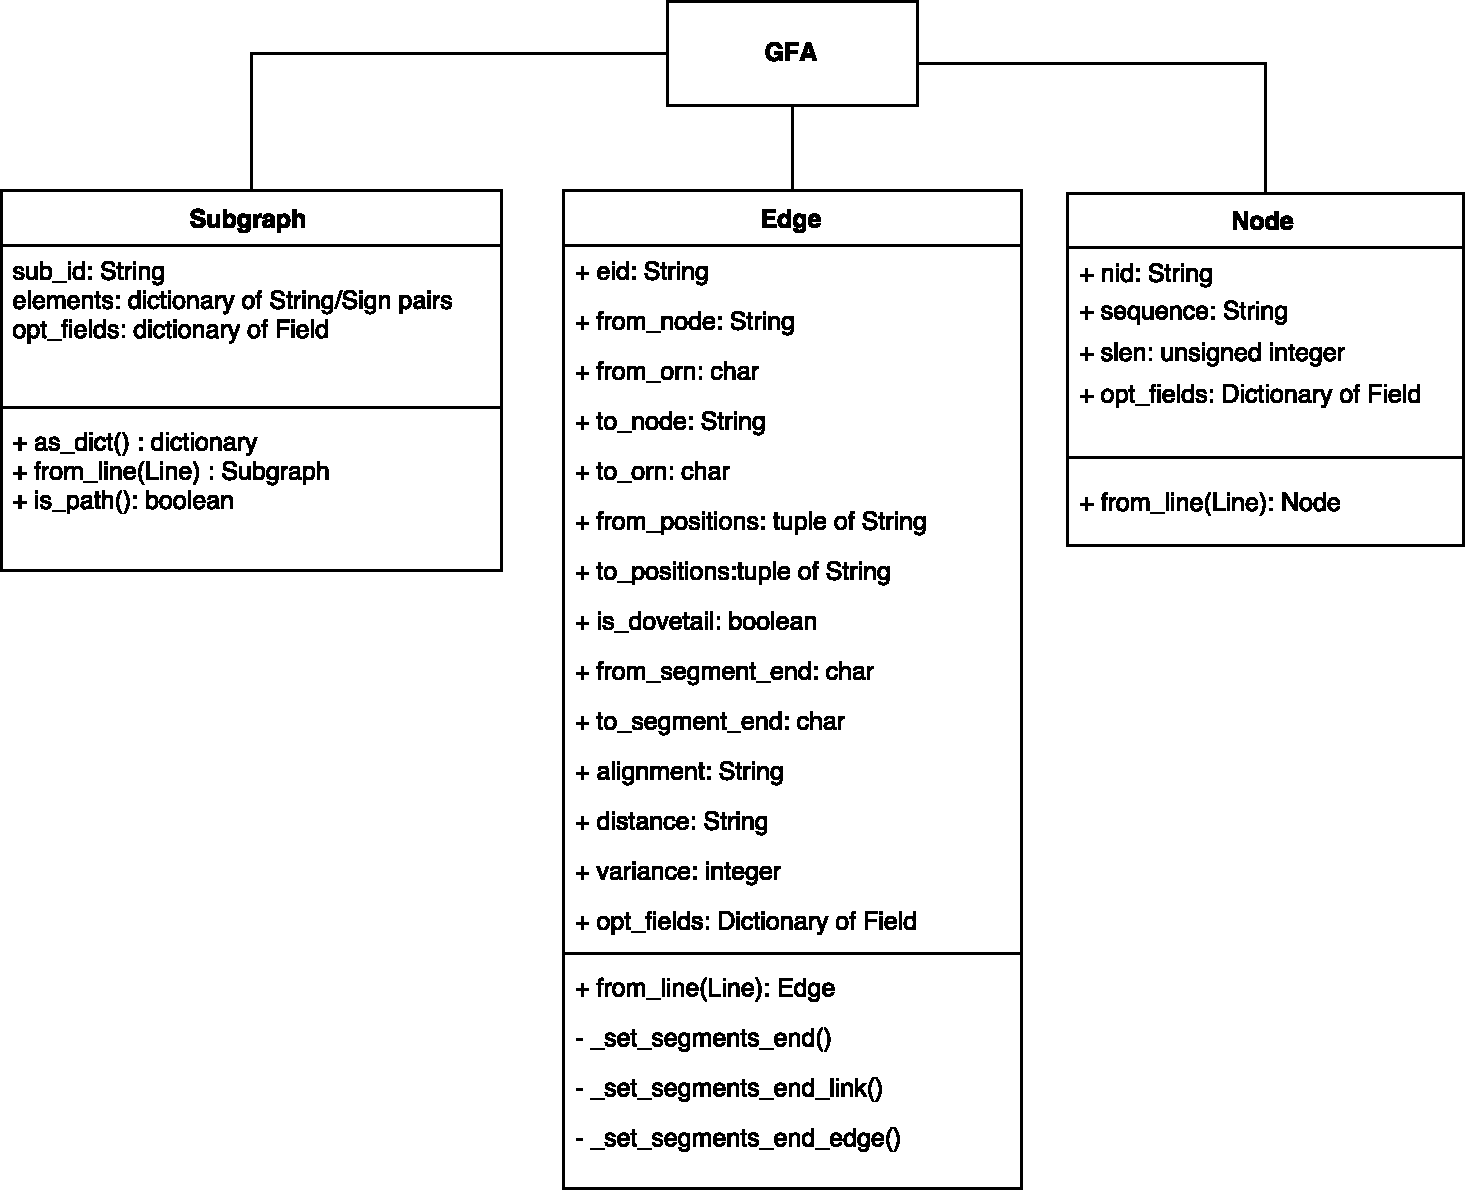
\includegraphics[scale=0.5]{graph_elements_class_diagram}
	\caption[Diagramma delle classi degli elementi del grafo]{Diagramma delle classi degli elementi del grafo.}
\end{figure}
\clearpage

\section{Fase3: rappresentazione del grafo GFA}
La classe che modella il grafo GFA sfrutta la classe Multigraph offerta
dalla libreria NetworkX come struttura ospitante gli archi e i nodi individuati
dalla fase precedente. Il multigrafo è stato scelto in quanto permette
di inserire più archi tra due nodi $u$ e $v$ inoltre
le relazioni presenti fra le sequenze non esprimono un senso di direzionalità
degli archi, perciò si è usato un grafo non diretto.
A nodi e archi è possibile inserire un qualsiasi tipo di riferimento ad un oggetto specificando
in fase di inserimento l'attributo del nodo al quale collegare il valore definito; la libreria
salverà l'informazione in un dizionario, di conseguenza il reperimento del valore
riferito al campo del nodo avverrà in modo analogo all'accesso ad un dizionario.

Per uniformarsi a tale comportamento \pygfa in fase creazione di nodi ed
archi estrapola gli attributi del elemento del grafo da inserire (in caso di nodo o arco)
e li inserisce sotto forma di coppia indice-valore di un dizionario. In questo modo
è possibile accedere facilmente ai diversi attributi di nodi e archi; inoltre
tale scelta è stata preferita in quanto questi elementi non hanno un comportamento,
ma rappresentano solamente un insieme di informazioni con relativi metodi di accesso.
di conseguenza sarebbe stato inappropriato descriverli mediante una classe.
\'E bene notare che ciò non vuole significare che le classi che modellano gli elementi
del grafo ricoprano un ruolo minore, esse sono servite ad astrarre informazioni
comuni ad elementi diversi tra loro riducendo quella complessità che altrimenti si
avrebbe avuto al momento di inserire nodi e archi nel grafo GFA.
I sottografi sono invece contenuti in un dizionario a parte, separato dalla struttura a
triplice dizionario rappresentata in figura \ref{fig:networkx-dict} a pagina \pageref{fig:networkx-dict};
il dizionario in questo caso contiene direttamente riferimenti ad oggetti Subgraph i quali
vengono convertiti in dizionari in base alle necessità dei metodi o dell'utente grazie
al metodo \texttt{as\_dict()}.

Per l'implementazione del grafo GFA si è scelto di usare la composizione al posto
di sfruttare l'ereditarietà della classe multigrafo. Tale scelta si è preferita per
un semplice concetto logico: la classe GFA \emph{sfrutta} un multigrafo senza
volerne emulare le funzionalità. Di conseguenza alla classe sono stati forniti i metodi di interfaccia
alla classe multigrafo oltre ad un metodo di accesso agli archi fornendo
solamente l'identificativo di un arco.

\subsection{Iteratore sugli archi di dovetail}
Come accennato a pagina \pageref{sec:link} le sovrapposizioni
che si sviluppano tra la fine di una sequenza e l'inizio di un'altra sono
informazioni di rilievo nel contesto dell'assemblaggio del genoma,
di conseguenza si è cercato di inserire una serie di meccanismi in \pygfa
che permettessero di distinguere gli archi che possiedono
il valore \texttt{is\_dovetail} a true, visto che NetworkX non fornisce
una soluzione a questa necessità (come descritto a pagina \pageref{sec:nx-why-limits}).

Questa funzionalità è stata implementata dalla classe \texttt{DovetailIterator} che
fornisce una serie di iteratori per scorrere i soli nodi del grafo collegati da archi di
dovetail overlap.
\noindent
\begin{figure}[t]
	\centering
	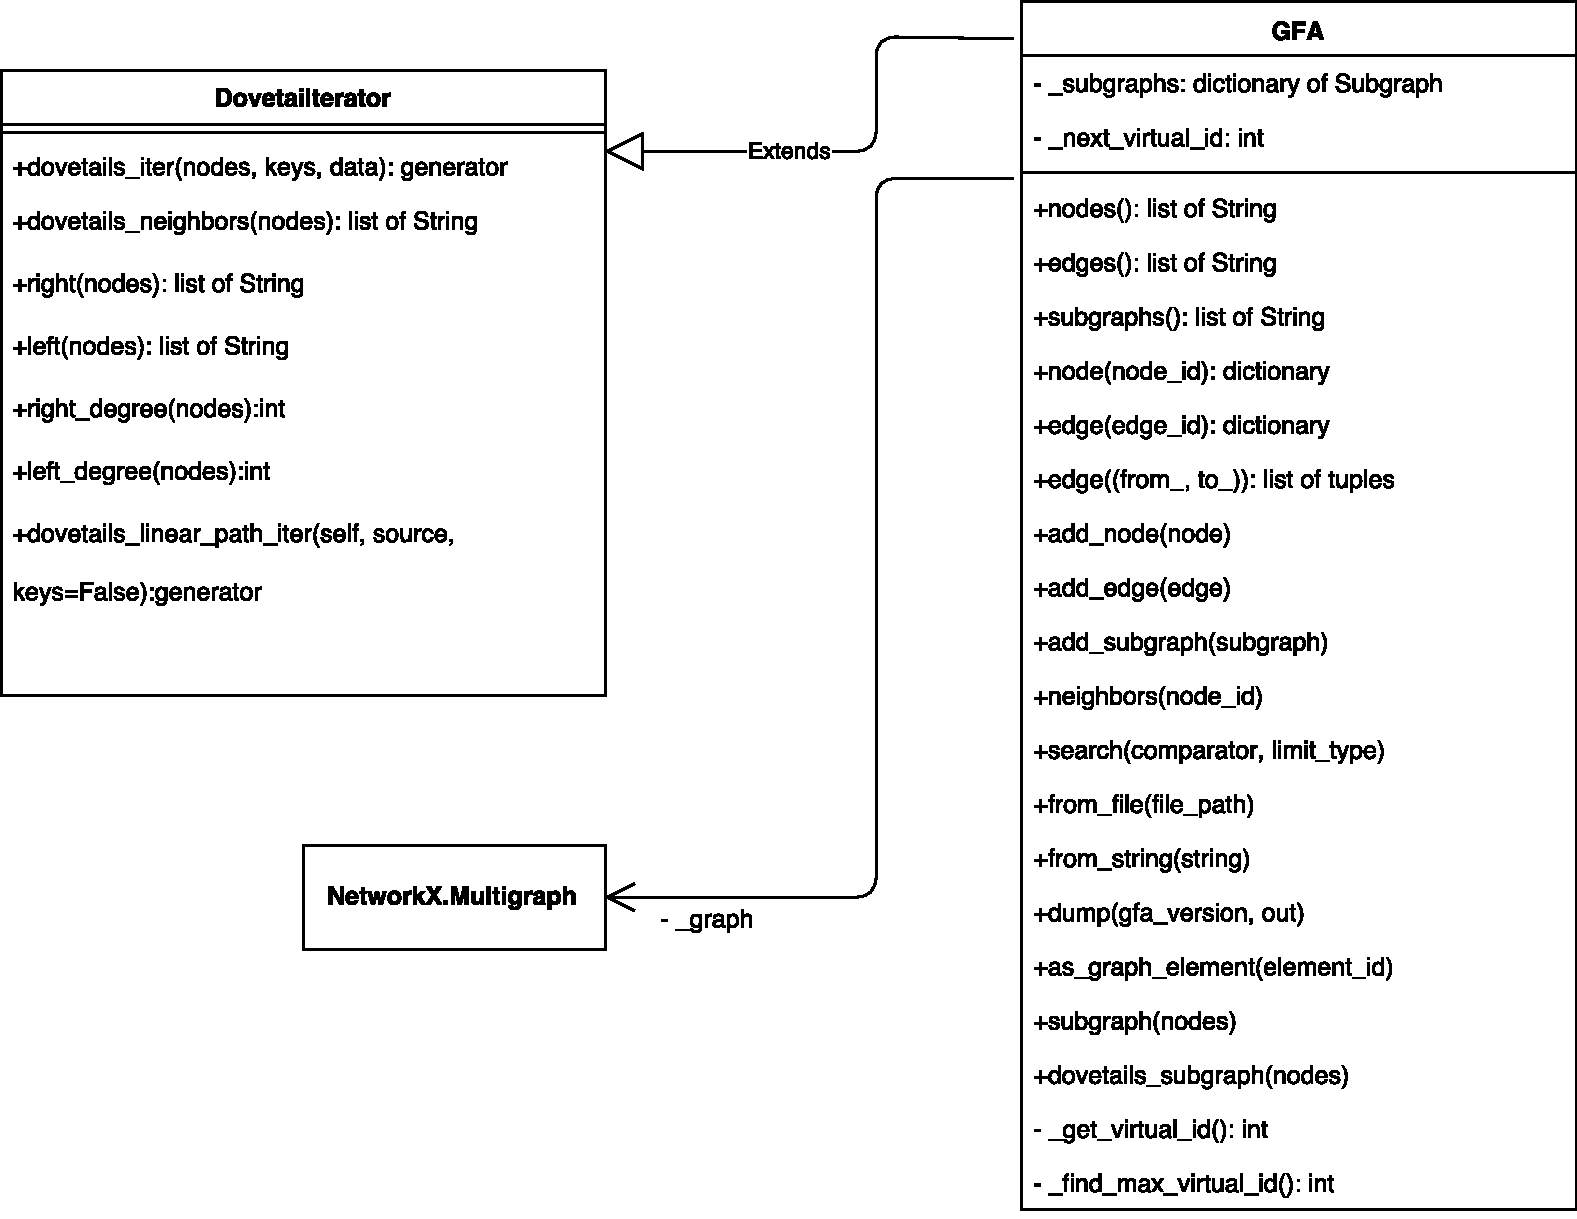
\includegraphics[scale=0.5]{gfa_class_diagram}
	\caption[Diagramma delle classi del grafo GFA]{Diagramma delle classi del grafo GFA.}
\end{figure}
\clearpage

\section{Operazioni sul grafo}
\pygfa offre una serie di operazioni che è possibile applicare sul grafo
composto da sequenze (nodi) e relazioni fra due sequenze (archi),
dividendole in due gruppi applicativi che si distinguono per le modalità
in cui gli archi vengono considerati nell'esecuzione delle operazioni.

Il primo insieme considera tutti gli archi del grafo, indistintamente dall'essere
archi di edge, fragment, gap o altro tipo. Queste operazioni sono
di utilità generale e servono per avere la massima flessibilità nella selezione delle
informazioni che il grafo contiene.

In questo gruppo troviamo il metodo della classe GFA \texttt{search} che
restituisce l'insieme di tutti gli elementi del grafo per i quali la funzione fornita
tra i parametri assume valore true. In questo modo l'utente definendo un
comparatore  può effettuare una serie di operazioni si ricerca e filtraggio sul grafo.

Inoltre, grazie all'uso della libreria NetworkX, è stato possibile con estrema facilità
creare delle interfacce ai metodi per l'individuazione delle componenti connesse, sia
per quanto riguarda la ricerca della componente connessa contente un nodo dato, che
la ricerca di tutte le componenti connesse presenti nel grafo.

Considerando l'alto livello di astrazione delle informazioni contenute
nel grafo, per l'utente che intende utilizzare \pygfa come strumento di
aiuto nella ricostruzione del genoma, è sconveniente andare ad eseguire
operazioni considerando archi che non sono di dovetail overlap, visto
che la relazione che essi descrivono è quella di maggior rilievo ai fini
dell'assemblaggio. Di conseguenza \pygfa come gfapy offre una serie
di operazioni che considerano esclusivamente archi di dovetail overlap.

\subsection{Operazioni sugli archi di dovetail overlap}
Gli algoritmi disponibili con NetworkX non permettono l'attraversamento
del grafo considerando le proprietà degli archi, non è quindi possibile
direttamente usare i metodi forniti come invece fatto per le operazioni
che considerano l'intero grafo (come già discusso a pagina \pageref{sec:nx-why-limits},
quando sono stati presentati i limiti della libreria). Nonostante questo inconveniente, vista
la natura open source di NetworkX e la licenza favorevole alla sua modifica
e distribuzione senza vincoli, è stato possibile modificare gli algoritmi necessari
per l'implementazione delle operazioni richieste. In tutti i casi l'unica modifica
richiesta per ottenere il risultato atteso consisteva nel modificare
l'elenco dei nodi considerati in fase di iterazione dell'algoritmo,
non più considerando l'intera lista di adiacenza del nodo selezionato
al ``livello'' corrente, ma prendendo in considerazione i nodi adiacenti
collegati da un arco di dovetail overlap. Visto che l'iteratore personalizzato
per l'attraversamento di questi archi è stato già sviluppato nella classe
DovetailIterator ed esteso dalla classe GFA, i metodi di iterazione
sono già forniti direttamente con il grafo GFA.

\noindent
\begin{lstlisting}[boxpos=t, numbers=left, language=Python, frame=t, caption=BFS in networkx., label=code:bfs-nx]
def _plain_bfs(G, source):
  G_adj = G.adj
  seen = set()
  nextlevel = {source}
    while nextlevel:
      thislevel = nextlevel
      nextlevel = set()
      for v in thislevel:
        if v not in seen:
          yield v
          seen.add(v)
          nextlevel.update(G_adj[v])
\end{lstlisting}

\captionsetup{justification=centering}
\begin{lstlisting}[boxpos=t, language=Python, numbers=left, frame=t, caption=BFS in \pygfa., label=code:bfs-pygfa]
def _plain_bfs_dovetails(gfa_, source):
  if source not in gfa_:
    return ()
  seen = set()
  nextlevel = {source}
  while nextlevel:
    thislevel = nextlevel
    nextlevel = set()
    for v in thislevel:
      if v not in seen:
        yield v
        seen.add(v)
        nextlevel.update(gfa_.right(v))
        nextlevel.update(gfa_.left(v))
\end{lstlisting}

I due listati rappresentano l'implementazione dell'algoritmo BFS (Breadth First Search) presente
nella libreria NetworkX (listato \ref{code:bfs-nx}) e l'equivalente implementato in \pygfa
(listato \ref{code:bfs-pygfa}). \'E possibile notare come l'unica differenza fra i due listati
è presente nella selezione dei nodi da considerare per la prossima iterazione, nelle ultime
righe di entrambi i listati; mentre in NetworkX viene considerata l'intera lista di adiacenza, in
\pygfa si sfruttano gli iteratori definiti in DovetailIterator per selezionare gli archi di dovetail overlap
presenti alle estremità del nodo.
Questo rappresenta una semplice modifica che si è dovuta effettuare per
implementare le operazioni di dovetail overlap, in alcuni casi le modifiche
hanno richiesto più tempo e l'analisi completa dell'operato dell'algoritmo (come nel
caso dell'algoritmo per la ricerca dei percorsi semplice fra due nodi),
ma nella maggior parte dei casi le modifiche richieste sono state semplici
ed intuitive.

Effettuando le modifiche sopra descritte è stato possibile sviluppare
le seguenti operazioni sugli archi di dovetail overlap:
\begin{itemize}
	\item ricerca delle componenti connesse;
	\item rimozione delle componenti connesse con lunghezza
		totale delle sequenze al di sotto di un determinato valore di soglia;
	\item rimozione delle estremità ``morte'', cioè tutti i nodi con
		grado di ingresso o uscita minore o uguale a 1 e la cui rimozione non causa
		la divisione di una componente connessa;
	\item ricerca degli insiemi di percorsi formati da unitig, cioè sequenze
		le cui estremità sono collegate ad una sola altra sequenza;
	\item ricerca di tutti i percorsi praticabili per arrivare da un nodo $u$ ad
		un nodo $v$.
\end{itemize}

\newpage
\section{Esempio}
Si andrà ora ad illustrare le funzionalità di \pygfa considerando il file GFA
contenente le informazioni nel listato \ref{code:gfa-es}, che visualizzato
con la libreria Matplotlib (strumento usato per la visualizzazione dell'intero grafo)
produce il risultato in figura \ref{fig:plot-matplot}; si sottolinea che tale libreria
considera il contesto biologico associato alle informazioni, ma visualizza
solamente gli elementi del grafo e la loro disposizione.
Per visualizzare il grafo con Bandage, in grado di visualizzare solo archi Link di GFA1,
il file GFA1 equivalente è stato ottenuto usando la funzione \texttt{dump}
di \pygfa, la quale è in grado di convertire le informazioni del grafo GFA
in una delle due specifiche.
Il risultato finale è in figura \ref{fig:plot-bandage}, si
può notare come i Gap (per esempio quello tra s8 ed s11)
non sono visualizzati da questo strumento.

\captionsetup{justification=centering, singlelinecheck=false}
\begin{minipage}{\linewidth}
\begin{lstlisting}[basicstyle=\ttfamily\scriptsize, frame=topline, label={code:gfa-es}, caption=Il file GFA2 usato per l'esempio.]
S	s1	10	*
S	s2	10	*
S	s3	10	*
S	s4	10	*
S	s5	10	*
S	s6	10	*
S	s7	10	*
S	s8	10	*
S	s9	10	*
S	s10	10	*
S	s11	10	*
S	s12	10	*
S	s13	10	*
S	s14	10	*
S	s15	10	*
S	s16	10	*
E	ls1s2	s1+	s2+	7	9$	0	2	*
E	ls2s4	s2+	s4+	7	9$	0	2	*
E	ls1s3	s1+	s3+	7	9$	0	2	*
E	ls3s5	s3+	s5+	7	9$	0	2	*
E	ls4s6	s4+	s6+	7	9$	0	2	*
E	ls5s6	s5+	s6+	7	9$	0	2	*
E	ls6s7	s6+	s7+	7	9$	0	2	*
E	ls7s8	s7+	s8+	7	9$	0	2	*
E	ls9s10	s9+	s10+	7	9$	0	2	*
E	ls11s12	s11+	s12+	7	9$	0	2	*
E	ls12s13	s12+	s13+	7	9$	0	2	*
E	ls14s15	s14+	s15+	7	9$	0	2	*
E	ls15s16	s15+	s16+	7	9$	0	2	*
E	ls16s14	s16+	s14+	7	9$	0	2	*
G	gs1s9	s1+	s9+	15	*
G	gs8s11	s8+	s11+	15	*
\end{lstlisting}
\end{minipage}
\captionsetup{justification=justified, singlelinecheck=false}

\captionsetup{justification=centering, singlelinecheck=false}
\begin{figure}
	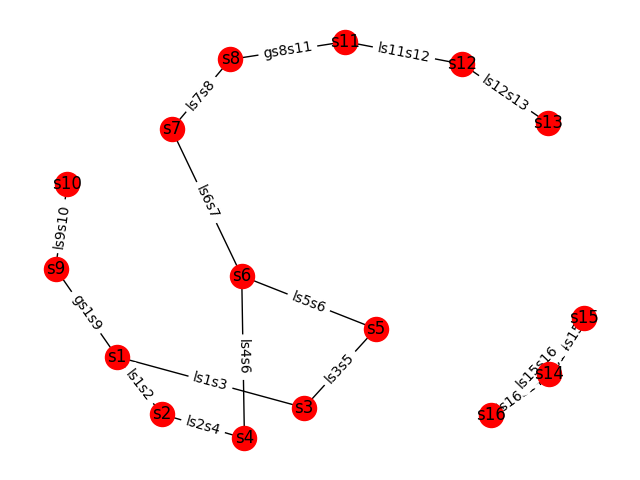
\includegraphics[scale=0.75]{matplot-es}
	\caption{Visualizzazione del grafo con matplotlib.}
	\label{fig:plot-matplot}
	\vspace{1cm}
	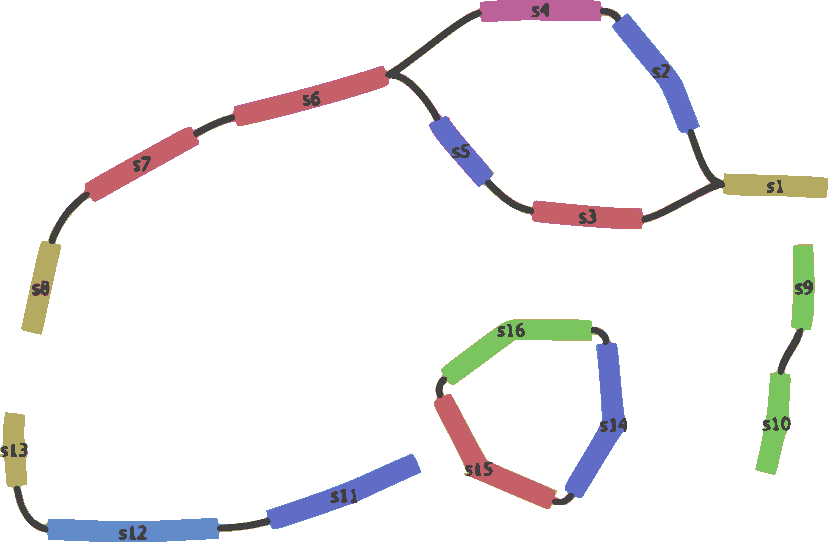
\includegraphics[scale=0.75]{bandage-es}
	\caption{Visualizzazione del grafo con Bandage.}
	\label{fig:plot-bandage}
\end{figure}
\captionsetup{justification=justified, singlelinecheck=false}

Caricato il grafo estraendo le informazioni dal file \texttt{gfa-es}
si andrà a presentare il modo in cui queste vengono rappresentate
mediante dizionari, si procederà successivamente
con la ricerca delle componenti connesse.
Si andrà ad illustrare l'operato degli iteratori personalizzati
cercando i segmenti collegati alle estremità di un nodo
specifico mediante l'uso i metodi \texttt{left} e \texttt{right}.
Si procederà quindi con le operazioni sugli archi di dovetail
individuando le componenti connesse e comparandole
con il risultato precedentemente ottenuto, per
poi concludere con i metodi per la ricerca
delle sequenze di unitig e dei cammini semplici
che si diramano tra due nodi $u$ e $v$.

\captionsetup{justification=centering, singlelinecheck=false}
\begin{minipage}{\linewidth}
\begin{lstlisting}[basicstyle=\ttfamily\scriptsize, frame=topline]
>>> import pygfa
>>> g = pygfa.gfa.GFA.from_file("..\..\gfa_es.gfa")
>>> g.nodes()
['s1', 's2', 's3', 's4', 's5', 's6', ..., 's15', 's16']
>>> g.node("s1")
{'nid': 's1', 'sequence': '*', 'slen': 10}
>>> g.edges(keys=True)
[('s1', 's2', 'ls1s2'), ('s1', 's3', 'ls1s3'), ..., ('s15', 's16', 'ls15s16')]
>>> g.edge(("s1", "s2"))
{'ls1s2': {'eid': 'ls1s2',
	'from_node': 's1', 'from_orn': '+', 'to_node': 's2', 'to_orn': '+',
	'from_positions': ('7', '9$'), 'to_positions': ('0', '2'),
	'alignment': '*', 'distance': None, 'variance': None,
	'is_dovetail': True, 'from_segment_end': 'R', 'to_segment_end': 'L'}}
>>> g.edge("ls1s2")
{'eid': 'ls1s2', 'from_node': 's1', 'from_orn': '+', 'to_node': 's2', 'to_orn': '+',
	'from_positions': ('7', '9$'), 'to_positions': ('0', '2'),
	'alignment': '*', 'distance': None, 'variance': None,
	'is_dovetail': True, 'from_segment_end': 'R', 'to_segment_end': 'L'}
>>> g.edge("ls1s2")["is_dovetail"]
True
\end{lstlisting}
\end{minipage}
\captionsetup{justification=justified, singlelinecheck=false}
La conversione degli elementi del grafo in dizionari ha permesso
una migliore integrazione nella libreria NetworkX facilitando l'accesso
alle informazioni del grafo. Di contro tale comportamento non permette di ricalcolare
automaticamente le informazioni della linea rappresentata in caso di modifica, cioè
non avendo una classe non è possibile attribuire un comportamento nella
gestione delle informazioni. Questo vuole significare che l'utente è libero di modificare
le informazioni, ma è suo compito assumersi la responsabilità che le modifiche
siano coerenti con il resto dei dati.


\captionsetup{justification=centering, singlelinecheck=false}
\begin{minipage}{\linewidth}
\begin{lstlisting}[basicstyle=\ttfamily\scriptsize, frame=topline, breaklines=true]
>>> pygfa.nodes_connected_components(g)
<generator object connected_components at ...>
>>>  le componenti connesse vengono restituite 
... # come generatore python
... # una componenente alla volta.
... # Per poterle visualizzare
... # tutte in una unica soluzione e'
... # necessario inserirle in una lista Python	
...
>>> list(pygfa.nodes_connected_components(g))
[
	{'s4', 's13', 's10', 's1', 's2',
		's3', 's9', 's5', 's8', 's12',
		's11', 's7', 's6'},
	{'s14', 's15', 's16'}
]
\end{lstlisting}
\end{minipage}
\captionsetup{justification=justified, singlelinecheck=false}
I due insiemi presenti all'interno della lista individuano le due componenti
connesse come mostra la figura \ref{fig:plot-matplot}. Tutti i tipi di archi che collegano
due nodi vengono presi in considerazione in tale operazione.


\captionsetup{justification=centering, singlelinecheck=false}
\begin{minipage}{\linewidth}
\begin{lstlisting}[basicstyle=\ttfamily\scriptsize, frame=topline]
>>> g.node("s1")
{'nid': 's1', 'sequence': '*', 'slen': 10}
>>> g.neighbors("s1")
['s2', 's3', 's9']
>>> g.right("s1")
['s2', 's3']
>>> g.left("s1")
[]
>>> g.dovetails_neighbors("s1")
['s2', 's3']
\end{lstlisting}
\end{minipage}
\captionsetup{justification=justified, singlelinecheck=false}
Dato il nodo $s1$ i nodi adiacenti considerando tutti i tipi di archi sono
dati dal metodo \texttt{neighbors}, mentre le operazioni successive
operano considerando solo archi di dovetail. Il metodo \texttt{left} restituisce
tutte le seguenze in cui è presente un dovetail overlap con la parte
sinistra della sequenza selezionata ($s1$ in questo caso), mentre il metodo
\texttt{right} restituisce le sequenze in cui la sovrapposizione avviene con
la parte destra della sequenza. I nodi adiacenti ad $s1$, considerando solo
questo tipo di collegamenti fra nodi, sono un sottoinsieme dei nodi individuati
dal metodo \texttt{neighbors}.


\captionsetup{justification=centering, singlelinecheck=false}
\begin{minipage}{\linewidth}
\begin{lstlisting}[basicstyle=\ttfamily\scriptsize, frame=topline]
>>> list(pygfa.dovetails_nodes_connected_components(g))
[
	{'s4', 's2', 's1', 's3', 's5', 's6', 's8', 's7'},
	{'s9', 's10'},
	{'s13', 's12', 's11'},
	{'s16', 's14', 's15'}
]
\end{lstlisting}
\end{minipage}
\captionsetup{justification=justified, singlelinecheck=false}
Le componenti connesse considerando gli archi di
dovetail sono più numerose rispetto quelle trovate
senza fare distinzione fra i legami dei nodi. Infatti si può
notare che gli archi di gap $(s9, s1)$ e $(s8, s13)$ non sono
presi in considerazione, facendo così aumentare il numero
totale delle componenti connesse. 


\captionsetup{justification=centering, singlelinecheck=false}
\begin{minipage}{\linewidth}
\begin{lstlisting}[basicstyle=\ttfamily\scriptsize, frame=topline]
>>> g.dovetails_linear_path_iter("s3")
<generator object DovetailIterator.dovetails_linear_path_traverse_edges_iter at ...>
>>> list(g.dovetails_linear_path_iter("s3"))
[('s3', 's5')]
>>> list(pygfa.dovetails_linear_paths(g))
[
	[('s4', 's2')],
	[('s15', 's14'), ('s14', 's16')],
	[('s13', 's12'), ('s12', 's11')],
	[('s9', 's10')],
	[('s5', 's3')],
	[('s7', 's8')]
]
>>> list(pygfa.dovetails_linear_paths(g, keys=True))
[
	[('s4', 's2', 'ls2s4')], 
	[('s15', 's14', 'ls14s15'), ('s14', 's16', 'ls16s14')],
	[('s13', 's12', 'ls12s13'), ('s12', 's11', 'ls11s12')],
	[('s9', 's10', 'ls9s10')],
	[('s5', 's3', 'ls3s5')],
	[('s7', 's8', 'ls7s8')]
]
\end{lstlisting}
\end{minipage}
\captionsetup{justification=justified, singlelinecheck=false}
L'iteratore sulle sequenze di unitig è un metodo
della classe GFA che restituisce gli archi che costituiscono il percorso
lineare contenente il nodo indicato come parametro.
La funzione per ricercare tutti i percorsi lineari sfrutta
gli iteratori sugli unitig per cercare l'insieme di tutte le sequenze
di unitig presenti nel grafo; alle tuple di nodi che compongono gli archi
che denotano i percorsi lineari è possibile associare anche il nome specifico
degli archi, in modo da distinguerli in presenza di più archi tra due nodi.


\captionsetup{justification=centering, singlelinecheck=false}
\begin{minipage}{\linewidth}
\begin{lstlisting}[basicstyle=\ttfamily\scriptsize, frame=topline]
>>> list(pygfa.dovetails_all_simple_paths(g, "s2", "s7"))
[
	['s2', 's1', 's3', 's5', 's6', 's7'],
	['s2', 's4', 's6', 's7']
]
>>> list(pygfa.dovetails_all_simple_paths(g, "s2", "s7", edges=True, keys=True))
[
	[('s2', 's1', 'ls1s2'), ('s1', 's3', 'ls1s3'),
		('s3', 's5', 'ls3s5'), ('s5', 's6', 'ls5s6'),
		('s6', 's7', 'ls6s7')],
	[('s2', 's4', 'ls2s4'), ('s4', 's6', 'ls4s6'),
		('s6', 's7', 'ls6s7')]
]
>>> list(pygfa.dovetails_all_simple_paths(g, "s2", "s11"))
[]
\end{lstlisting}
\end{minipage}
\captionsetup{justification=justified, singlelinecheck=false}
Nell'esempio si vogliono trovare tutti i percorsi che congiungono
il nodo $s2$ al nodo $s7$, la funzione ritorna le liste dei nodi che individuano
i percorsi di congiunzione. Impostando l'attributo \texttt{edges}
a True la funzione ritorna le sequenze di archi dei percorsi.
Nel caso non sia presente un percorso fra i due nodi specificati, la funzione
ritorna un generatore privo di elementi, che viene convertito
dalla funzione \texttt{list} in una lista vuota.
